\documentclass{beamer}
\usetheme{Madrid} % Tema elegante y profesional
\usecolortheme{default} % Colores neutros
\usepackage[utf8]{inputenc}
\usepackage{amsmath}
\usepackage{graphicx}
\usepackage[spanish]{babel}

\title{Modelo Matemático para la Bioconversión de Residuos por Larvas de Mosca Soldado Negra}
\author{John Leal}
\institute{Universidad Nacional de Colombia}
\date{\today}

\begin{document}

% Diapositiva de título
\begin{frame}
    \titlepage
\end{frame}

% Introducción
\begin{frame}{Introducción}
    \begin{itemize}
        \item El modelo describe el proceso de bioconversión de residuos orgánicos mediante larvas de mosca soldado negra (\textit{Hermetia illucens}).
        \item Objetivo: Determinar la cantidad de dióxido de carbono ($CO_2$) generada durante el proceso.
        \item Se utilizan suposiciones simplificadoras basadas en cinética tipo Monod.
    \end{itemize}
\end{frame}

% Suposiciones del Modelo
\begin{frame}{Suposiciones del Modelo}
    \begin{itemize}
        \item La biomasa de residuos disminuye debido al consumo por parte de las larvas.
        \item El crecimiento larvario depende de la disponibilidad de residuos (cinética tipo Monod).
        \item La producción de $CO_2$ está directamente relacionada con el consumo de residuos.
        \item Los residuos se convierten en biomasa larvaria y $CO_2$ con rendimientos específicos.
        \item Condiciones ambientales son óptimas y constantes.
    \end{itemize}
\end{frame}

% Variables y Parámetros Clave
\begin{frame}{Variables y Parámetros Clave}
    \begin{itemize}
        \item $B(t)$: Biomasa de residuos disponibles [g].
        \item $L(t)$: Biomasa total de larvas [g].
        \item $C(t)$: Cantidad acumulada de $CO_2$ producida [g].
        \item $\mu_L$: Tasa máxima específica de consumo de residuos [g residuo / g larva / día].
        \item $K_B$: Constante de saturación de residuos [g].
        \item $Y_{L/B}$: Rendimiento de biomasa larvaria por unidad de residuo consumido [g larva / g residuo].
        \item $Y_{C/B}$: Rendimiento de $CO_2$ por unidad de residuo consumido [g $CO_2$ / g residuo].
        \item $L_{max}$: Biomasa larvaria máxima sostenible [g].
    \end{itemize}
\end{frame}

% Ecuaciones Diferenciales
\begin{frame}{Ecuaciones Diferenciales del Modelo}
    \begin{itemize}
        \item Consumo de residuos:
        \[
        \frac{dB}{dt} = -\mu_L \cdot \frac{B(t)}{K_B + B(t)} \cdot L(t)
        \]
        \item Crecimiento larvario:
        \[
        \frac{dL}{dt} = Y_{L/B} \cdot \mu_L \cdot \frac{B(t)}{K_B + B(t)} \cdot L(t) \cdot \left(1 - \frac{L(t)}{L_{max}}\right)
        \]
        \item Producción de $CO_2$:
        \[
        \frac{dC}{dt} = Y_{C/B} \cdot \mu_L \cdot \frac{B(t)}{K_B + B(t)} \cdot L(t)
        \]
    \end{itemize}
\end{frame}

% Resultados Numéricos
\begin{frame}{Resultados Numéricos}
    \begin{itemize}
        \item Ejemplo con parámetros:
        \begin{itemize}
            \item $B_0 = 500$ g, $L_0 = 10$ g, $\mu_L = 0.08$, $K_B = 20$ g, $Y_{L/B} = 0.4$, $Y_{C/B} = 1.8$, $L_{max} = 200$ g.
            \item Después de 10 días:
            \begin{itemize}
                \item Residuos consumidos: 400 g.
                \item Biomasa larvaria final: 80 g.
                \item $CO_2$ producido: 720 g.
            \end{itemize}
        \end{itemize}
    \end{itemize}
\end{frame}
\begin{frame}{Simulación}
\begin{figure}[htbp]
    \centering
    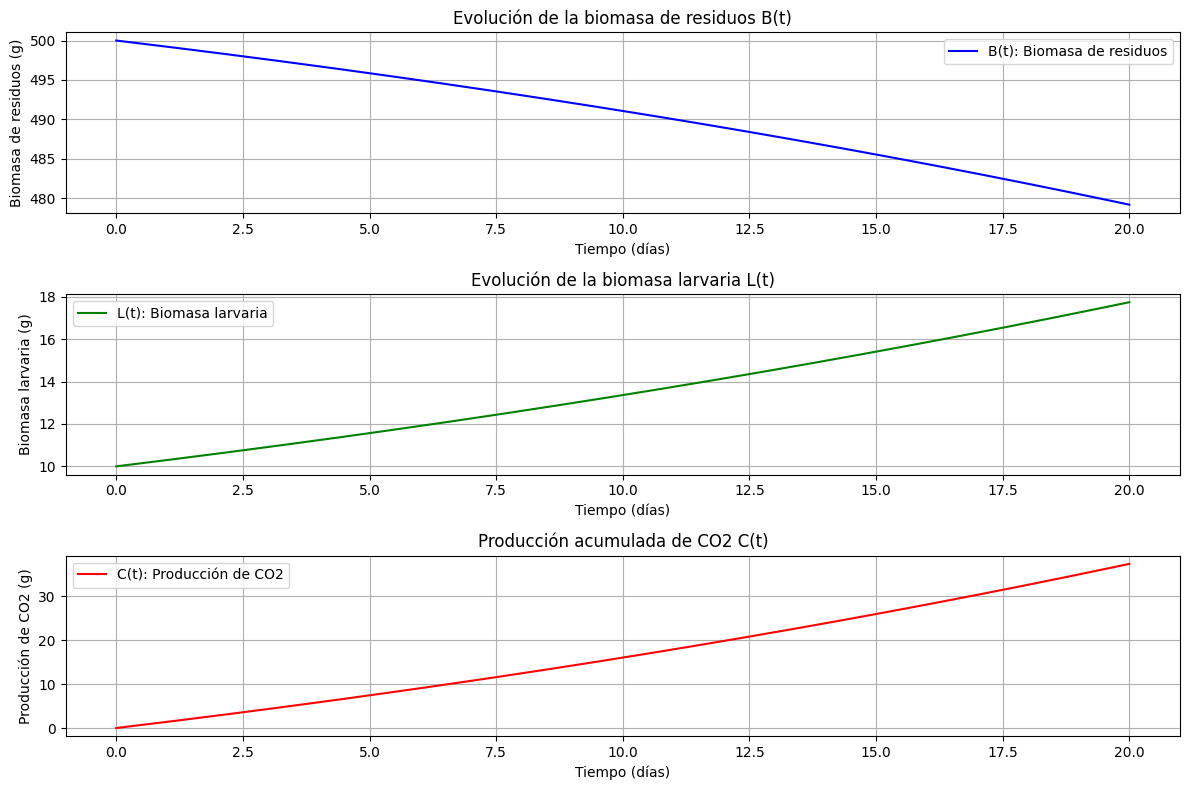
\includegraphics[width=0.8\textwidth]{solucion_ecuaciones.png} % Cambia "grafica.png" por el nombre de tu archivo
    \caption{Evolución de la biomasa de residuos ($B(t)$), biomasa larvaria ($L(t)$) y producción de $CO_2$ ($C(t)$).}
    \label{fig:resultados}
\end{figure}

\end{frame}

% Conclusiones
\begin{frame}{Conclusiones}
    \begin{itemize}
        \item El modelo permite predecir la dinámica del proceso de bioconversión.
        \item Útil para optimizar sistemas de bioconversión y evaluar su impacto ambiental.
        \item Importancia de los parámetros como $\mu_L$, $K_B$, $Y_{L/B}$, $Y_{C/B}$ y $L_{max}$.
        \item Herramienta clave para estudios experimentales y aplicaciones prácticas.
    \end{itemize}
\end{frame}

% Referencias
\begin{frame}{Referencias}
    \begin{itemize}
        \item Diener, S., et al. (2011). Biological treatment of municipal organic waste using black soldier fly larvae. \textit{Waste and Biomass Valorization}.
        \item Shuler, M. L., et al. (2017). \textit{Bioprocess Engineering: Basic Concepts}. Pearson.
    \end{itemize}
\end{frame}

\end{document}
